% =====================================================================
%  Slide-Examiner --- AAAI-27 Technical Supplement (anonymized)
%  Build:  pdflatex supplement && pdflatex supplement   (no bibtex)
%  Self-contained extension of the main paper. Referenced from the body
%  for the SlideAudit crosswalk, the full multi-reward audit grid, the
%  full examiner table, and the extended figures omitted for space.
% =====================================================================
\documentclass[11pt]{article}
\usepackage[T1]{fontenc}
\usepackage[utf8]{inputenc}
\usepackage{amsmath,amssymb}
\usepackage{newtxtext,newtxmath}
\usepackage[margin=1in]{geometry}
\usepackage{microtype}
\usepackage{graphicx}
\usepackage{booktabs}
\usepackage{array}
\usepackage{multirow}
\usepackage[table]{xcolor}
\usepackage[percent]{overpic}
\usepackage{caption}
\captionsetup{font=small,labelfont=bf,skip=4pt}
\usepackage[colorlinks=true,linkcolor=NavyBlue,citecolor=NavyBlue,urlcolor=NavyBlue]{hyperref}
\definecolor{NavyBlue}{RGB}{31,90,135}
\definecolor{figink}{HTML}{2B3440}
\definecolor{figslate}{HTML}{5A6675}
\definecolor{figblue}{HTML}{3F6FB5}
\definecolor{figorange}{HTML}{E07F2C}
\definecolor{figred}{HTML}{D24A43}
\definecolor{figgrey}{HTML}{9AA4B0}

\newcommand{\g}[1]{\textsf{#1}}
\newcommand{\best}[1]{\textbf{#1}}
\newcommand{\ci}[1]{\,{\scriptsize[#1]}}

\title{\bf Technical Supplement:\\
``It's the Elicitation, Not the Eyes: Diagnosing VLM Failures in Slide
Quality Inspection and Routing a Symbolic--Neural Critic''}
\author{Anonymous Authors (AAAI-27 Submission)}
\date{}

\begin{document}
\maketitle

This supplement extends the main paper with material referenced from the body
but omitted there for space: the SlideAudit crosswalk (\S\ref{app:crosswalk}),
the full multi-reward / VLM-judge audit grid with per-class preference accuracies
(\S\ref{app:reward}), the full page-semantic examiner table including the
deck-scope negative result (\S\ref{app:examiner}), and the extended figures
(\S\ref{app:figs}). All numbers are transcribed verbatim from the frozen
analysis reports and rollout CSVs that accompany this submission as the Code
and Data Supplement; no new claim is made here.

% =====================================================================
\section{SlideAudit crosswalk}\label{app:crosswalk}
% =====================================================================

Table~\ref{tab:slideaudit-crosswalk} gives the bidirectional map between our
G/S defect classes and the 19-dimensional expert-derived \textsc{SlideAudit}
taxonomy, referenced from \S3 of the main paper. Empty entries are intentional
off-taxonomy semantic or deck-level defects; \g{G7} refines, rather than
duplicates, \textsc{SlideAudit}'s content-overflow/cut-off category by adding
the declared-legal-box criterion that makes the defect linter-blind.

\begin{table}[h]
\centering
\footnotesize
\setlength{\tabcolsep}{3pt}
\caption{Crosswalk between our G/S classes and the 19-dimensional \textsc{SlideAudit} taxonomy.}
\label{tab:slideaudit-crosswalk}
\begin{tabular}{@{}p{0.20\linewidth}p{0.42\linewidth}p{0.30\linewidth}@{}}
\toprule
Our class & \textsc{SlideAudit} class & Relation \\
\midrule
\g{G1} text overflow & Content Overflow/Cut-off & equivalent \\
\g{G2} element overlap & Occluded Content & equivalent \\
\g{G3} alignment offset & Content Alignment Issues & equivalent \\
\g{G4} font-size inconsistency & Improper Font Sizing & equivalent \\
\g{G5} brand-color violation & Excessive or Inconsistent Color Usage; Inappropriate or Mismatched Color Combinations & equivalent \\
\g{G6} margin violation & Unbalanced Space Distribution & near-equivalent; safe-margin bleed is a special case \\
\g{G7} render-containment overflow & Content Overflow/Cut-off; related to Improper Image Sizing & our extension; same visual symptom plus declared-legal-box criterion \\
\g{S1} title/body mismatch & -- & off-taxonomy content semantics \\
\g{S2} narrative-order break & -- & off-taxonomy deck-level ordering \\
\g{S3} terminology inconsistency & -- & off-taxonomy cross-slide terminology \\
\g{S4} density violation & Excessive Text Volume & equivalent \\
\g{S5} missing logic section & -- & off-taxonomy deck-level completeness \\
\g{S6} image/text contradiction & Irrelevant Visual Content (nearest) & nearest only; contradiction rather than relevance \\
\bottomrule
\end{tabular}
\end{table}

% =====================================================================
\section{Full multi-reward / VLM-judge audit grid}\label{app:reward}
% =====================================================================

Table~\ref{tab:reward-full} expands the main paper's Table~3 (which reports
only \g{G5} and \g{G7}) to the full per-class paired preference accuracy
$P(r_{\text{clean}}>r_{\text{def}})$ for all audited classes, with 95\% CIs on
\g{G7}. Each scorer penalizes several in-taxonomy defects it can see,
confirming each is a functioning scorer rather than a domain mismatch; the
\g{G7} column is the linter-blind render class whose detection splits the
scorers by perceptual capability, not training domain
(\S5.3 of the main paper). Per-cell precision and the full multiplicity
report (61 paired tests with Holm/Benjamini--Hochberg correction) are in the
Code and Data Supplement (\texttt{reports/}).

\begin{table}[h]
\centering
\small
\setlength{\tabcolsep}{4pt}
\caption{Multi-reward / VLM-judge audit: paired preference accuracy per class
(chance $=0.5$; \g{G7} with 95\% CI). \checkmark/$\times$ marks reliable \g{G7}
detection (CI above / spanning 0.5). \g{G5} is the internal-chromatic
re-operationalisation of \S4, a \emph{visible} defect most scorers catch, not
the linter-only blind spot \g{G7} is.}
\label{tab:reward-full}
\begin{tabular}{@{}llccc>{\columncolor[gray]{0.92}}c cc@{}}
\toprule
Reward scorer & category & \g{G1} & \g{G2} & \g{G5} & \textbf{\g{G7}} & \g{S4} & \g{S6} \\
\midrule
DocReward-3B   & document   & 0.93 & 1.00 & 0.72 & $\times$\,\textbf{0.48}\,{\scriptsize$[.38,.58]$} & 1.00 & 1.00 \\
\midrule
Skywork-VL-7B  & general-mm & 0.94 & 0.72 & 0.57 & \checkmark\,\textbf{0.79}\,{\scriptsize$[.69,.86]$} & 0.92 & 1.00 \\
PickScore-v1   & general-mm & 0.74 & 0.59 & 0.70 & \checkmark\,\textbf{0.71}\,{\scriptsize$[.61,.80]$} & 1.00 & 0.72 \\
\midrule
LAION-Aesth.   & aesthetic  & 0.37 & 0.91 & 0.78 & $\times$\,\textbf{0.57}\,{\scriptsize$[.46,.66]$} & 0.75 & 0.61 \\
CLIP-IQA       & aesthetic  & 0.44 & 0.50 & 0.65 & \checkmark\,\textbf{0.83}\,{\scriptsize$[.74,.90]$} & 0.50 & 0.72 \\
\midrule
Qwen3.7-Max judge & frontier VLM & 0.13 & 0.92 & -- & \checkmark\,\textbf{1.00}\,{\scriptsize$[.86,1]$} & 1.00 & -- \\
\midrule
\multicolumn{2}{@{}l}{$n$ (paired; non-VLM rows)} & 54 & 54 & 80 & 90 & 36 & 18 \\
\multicolumn{2}{@{}l}{$n$ (Qwen3.7-Max judge row)} & 24 & 24 & -- & 24 & 24 & -- \\
\bottomrule
\end{tabular}
\end{table}

% =====================================================================
\section{Full page-semantic examiner table}\label{app:examiner}
% =====================================================================

Table~\ref{tab:examiner-full} reproduces the page-semantic inspection table
of \S6 of the main paper, here shown with the deck-scope \g{S2}/\g{S5}
negative result and the full per-cell context.

\begin{table}[h]
\centering
\small
\caption{Page-semantic inspection, balanced accuracy [95\% Wilson] on paired
clean (best modality). The finetuned 8B examiner beats both zero-shot
baselines, including the 30B, \emph{in-distribution}. Deck-scope \g{S2}/\g{S5}
are a negative result. $n$ = paired positives (2-AFC rows = forced-choice
pairs); the \g{S6} 2-AFC rests on only 12 pairs and is descriptive only.}
\label{tab:examiner-full}
\begin{tabular}{@{}lcccr@{}}
\toprule
class & \textbf{ft-8B} & zs-8B & zs-30B & $n$ \\
\midrule
\g{S1} title/body  & \best{1.000}\ci{.95,1} & 0.778\ci{.69,.85} & 0.933\ci{.87,.95} & 36 \\
\g{S4} density     & \best{1.000}\ci{.97,1} & 0.529\ci{.50,.58} & 0.774\ci{.69,.84} & 60 \\
\g{G1} overflow (2-AFC) & \best{1.000}\ci{.97,1} & 0.975\ci{.93,.99} & 0.700\ci{.61,.77} & 120 \\
\g{S6} image/text (2-AFC) & \best{1.000}\ci{.76,1} & 1.000\ci{.76,1} & 0.500\ci{.25,.75} & 12 \\
\midrule
\g{S2} narrative (deck) & 0.500$^\dagger$\ci{.45,.53} & 0.646\ci{.53,.72} & 0.549\ci{.42,.66} & 36 \\
\g{S5} missing-logic (deck) & 0.500\ci{.47,.53} & 0.500\ci{.47,.53} & 0.567\ci{.45,.68} & 60 \\
\bottomrule
\end{tabular}
\\[2pt]
{\footnotesize $^\dagger$ degenerate (always-flag): the SFT mix had no
clean-\emph{deck} negatives. See \S6 of the main paper.}
\end{table}

% =====================================================================
\section{Human spot-check v2}\label{app:spotcheckv2}
% =====================================================================

The rebuilt-corpus human spot-check used in the revised limitations text is
summarised in Table~\ref{tab:spotcheck-v2}. To avoid rewriting the full 69-pair
sample for a definition bug confined to legacy \g{G3}/\g{G5}, we kept the other
55 pairs fixed and replaced only those stale samples with corrected internal-
contrast variants (within-list misalignment for \g{G3}, within-list chromatic
clash for \g{G5}). The resulting v2 sample has 73 pairs. The paired clean
controls remain clean throughout, and the source-structure faithfulness audit on
the auditable classes is 55/55 (see \texttt{data/part3/e8\_ir\_faithfulness\_v2.json}
in the Code and Data Supplement). A short delta summary is provided in
\texttt{reports/\_e8\_spotcheck\_v2\_delta.md}.

\begin{table}[h]
\centering
\small
\caption{Human spot-check v2 on the rebuilt corpus. Rates are human
perceptual-verification rates on the defective render and clean-twin
verification rates on the paired clean render.}
\label{tab:spotcheck-v2}
\setlength{\tabcolsep}{4pt}
\begin{tabular}{@{}lccc@{}}
\toprule
class & defect visible & twin clean & $n$ \\
\midrule
\g{G1} & 1.00\ci{.70,1} & 1.00\ci{.70,1} & 9 \\
\g{G2} & 1.00\ci{.65,1} & 1.00\ci{.65,1} & 7 \\
\g{G3} & 1.00\ci{.68,1} & 1.00\ci{.68,1} & 8 \\
\g{G5} & 1.00\ci{.72,1} & 1.00\ci{.72,1} & 10 \\
\g{G6} & 1.00\ci{.65,1} & 1.00\ci{.65,1} & 7 \\
\g{G7} & 1.00\ci{.70,1} & 1.00\ci{.70,1} & 9 \\
\g{S1} & 1.00\ci{.65,1} & 1.00\ci{.65,1} & 7 \\
\g{S4} & 1.00\ci{.65,1} & 1.00\ci{.65,1} & 7 \\
\g{S6} & 1.00\ci{.70,1} & 1.00\ci{.70,1} & 9 \\
\midrule
\textbf{overall} & \textbf{1.00\ci{.95,1}} & \textbf{1.00\ci{.95,1}} & \textbf{73} \\
\bottomrule
\end{tabular}
\end{table}

% =====================================================================
\section{Extended figures}\label{app:figs}
% =====================================================================

These figures were omitted from the main paper for space; their findings are
stated in the body prose. They are included here for completeness.

\begin{figure}[h]
\centering
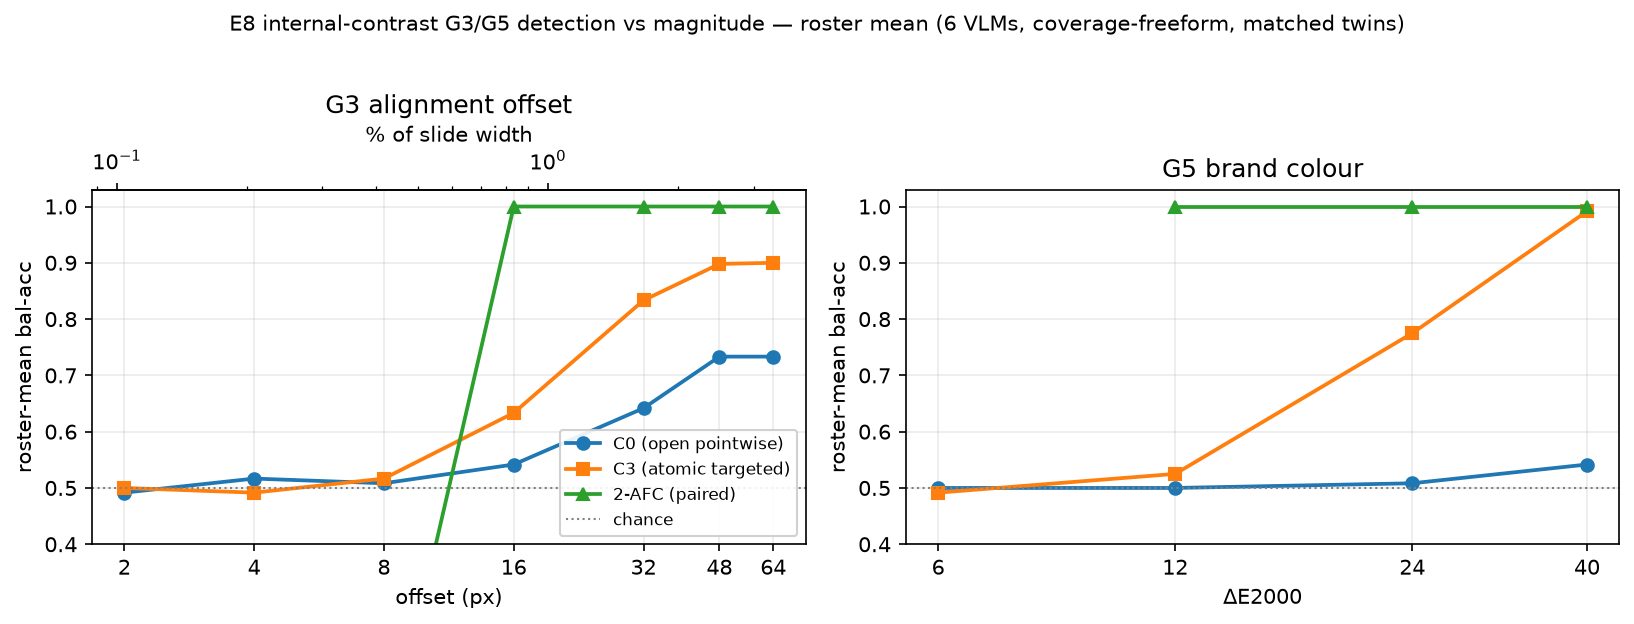
\includegraphics[width=0.85\linewidth]{figs/fig10_g3_saturation.png}
\caption{\textbf{Fine geometry is magnitude-gated, not a flat capability floor}
(referenced as the saturation curve in \S4). Roster-mean balanced accuracy
(6 VLMs, matched-twin internal-contrast set) vs.\ injected magnitude for
\g{G3} alignment (left) and \g{G5} brand color (right). Open pointwise (C0)
lags; atomic targeted (C3) recovers to $\approx0.90$ by $48$--$64$\,px /
$0.99$ by $\Delta E\,40$; the paired 2-AFC saturates to $1.00$ by $16$\,px
($0.83\%$) / $\Delta E\,12$. The sub-threshold tail ($\le8$\,px,
$\le6\,\Delta E$) stays at chance under every protocol.}
\label{figA:sat}
\end{figure}

\begin{figure}[h]
\centering
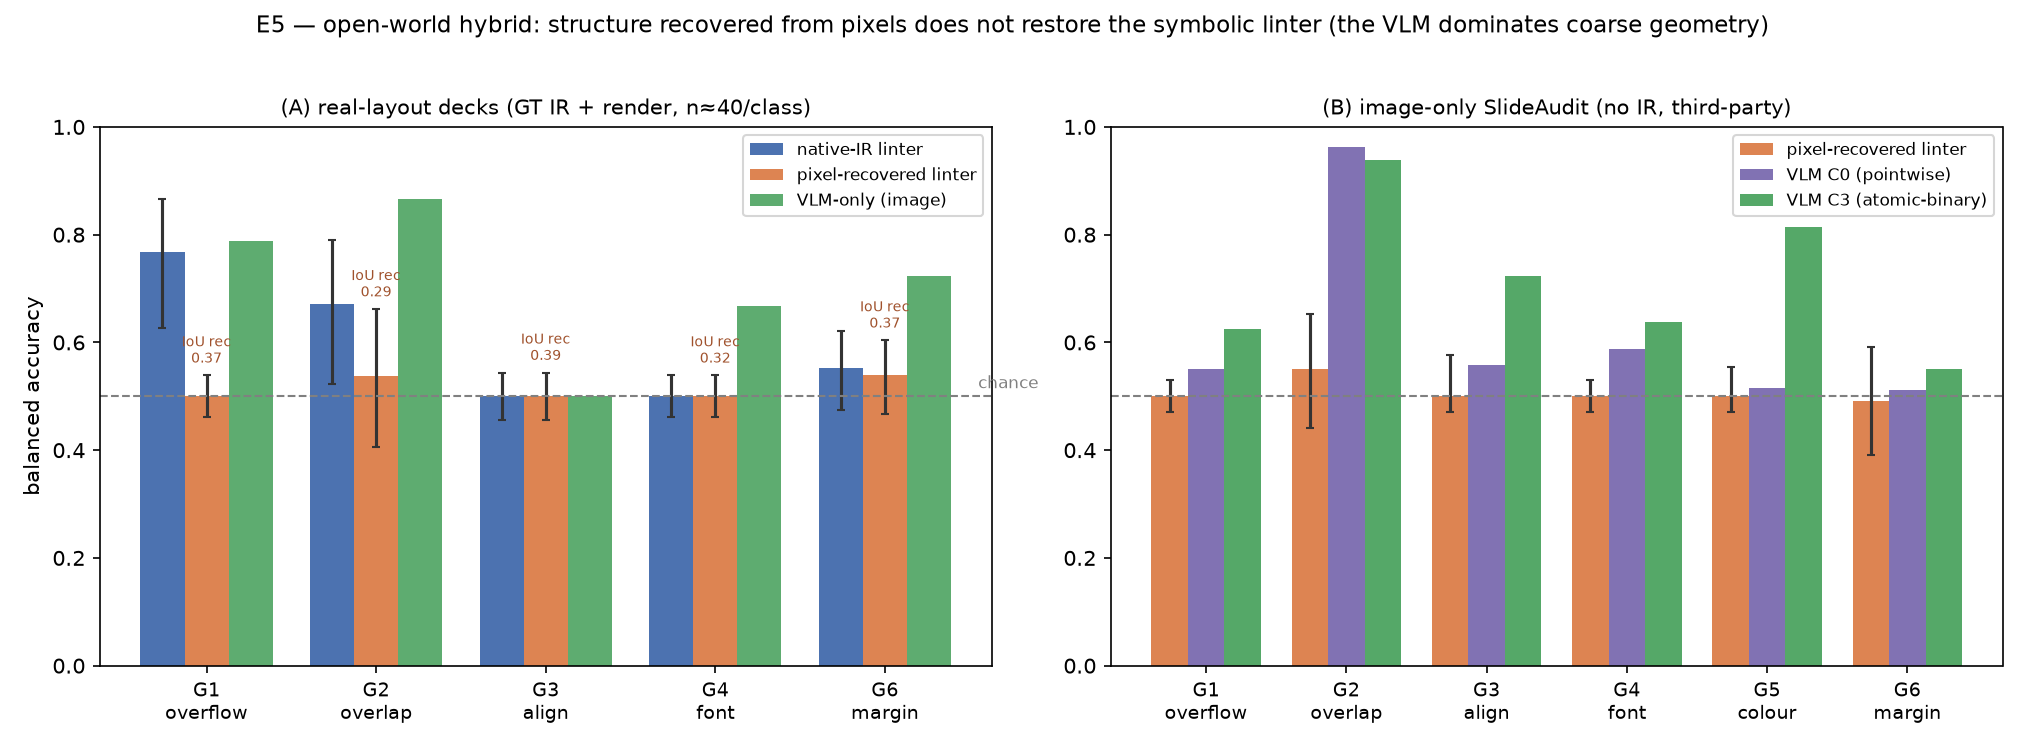
\includegraphics[width=0.85\linewidth]{figs/fig8_open_world_recovery.png}
\caption{\textbf{Open-world hybrid: structure recovered from pixels does not
restore the symbolic linter} (referenced in \S7). \textbf{(A)} real-layout
decks (GT IR + render, $n{\approx}40$/class): native-IR linter vs.\
pixel-recovered linter vs.\ VLM-only floor, Wilson CIs; recovered structure
rescues only overlap (\g{G2}) and is silent on fine geometry, while the VLM
dominates every class. \textbf{(B)} image-only \textsc{SlideAudit} (no IR,
third-party): the recovered linter clears chance only on \g{G2}; the
C3-elicited VLM is far stronger.}
\label{figA:openworld}
\end{figure}

\begin{figure}[h]
\centering
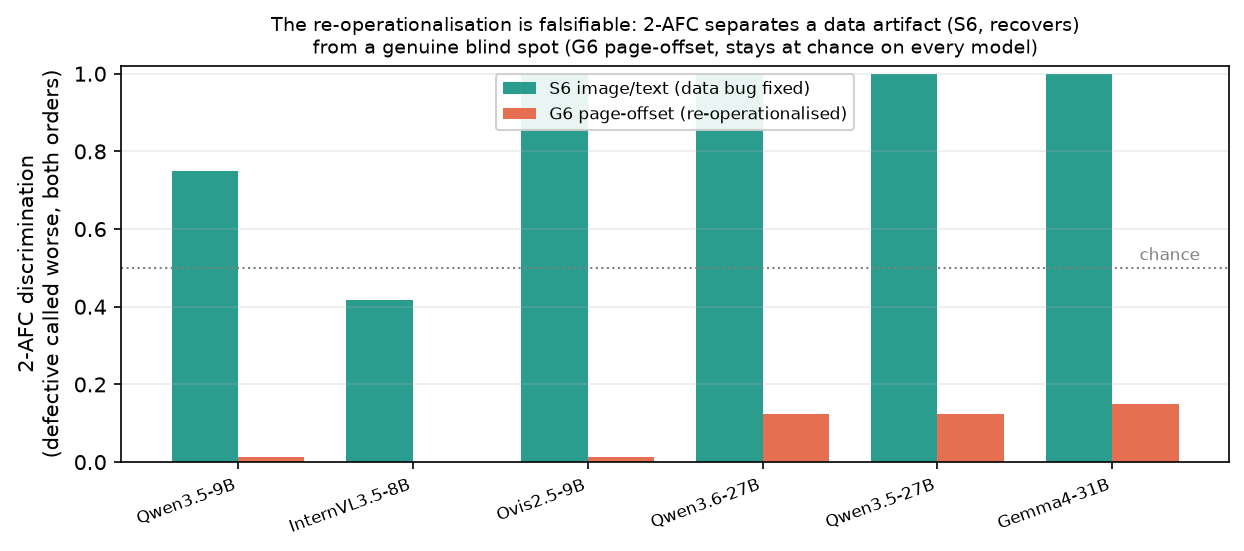
\includegraphics[width=0.75\linewidth]{figs/fig11_artifact_vs_genuine.png}
\caption{\textbf{A genuine blind spot the forced choice exposes} (referenced
in \S4). Per-model 2-AFC discrimination. Pointwise puts both classes at
chance, but the forced choice \emph{separates} them: the data artifact \g{S6}
recovers on every model, while \g{G6} page offset stays at the floor on every
model---a genuine blind spot, not an elicitation or data artifact.}
\label{figA:artifact}
\end{figure}

\begin{figure}[h]
\centering
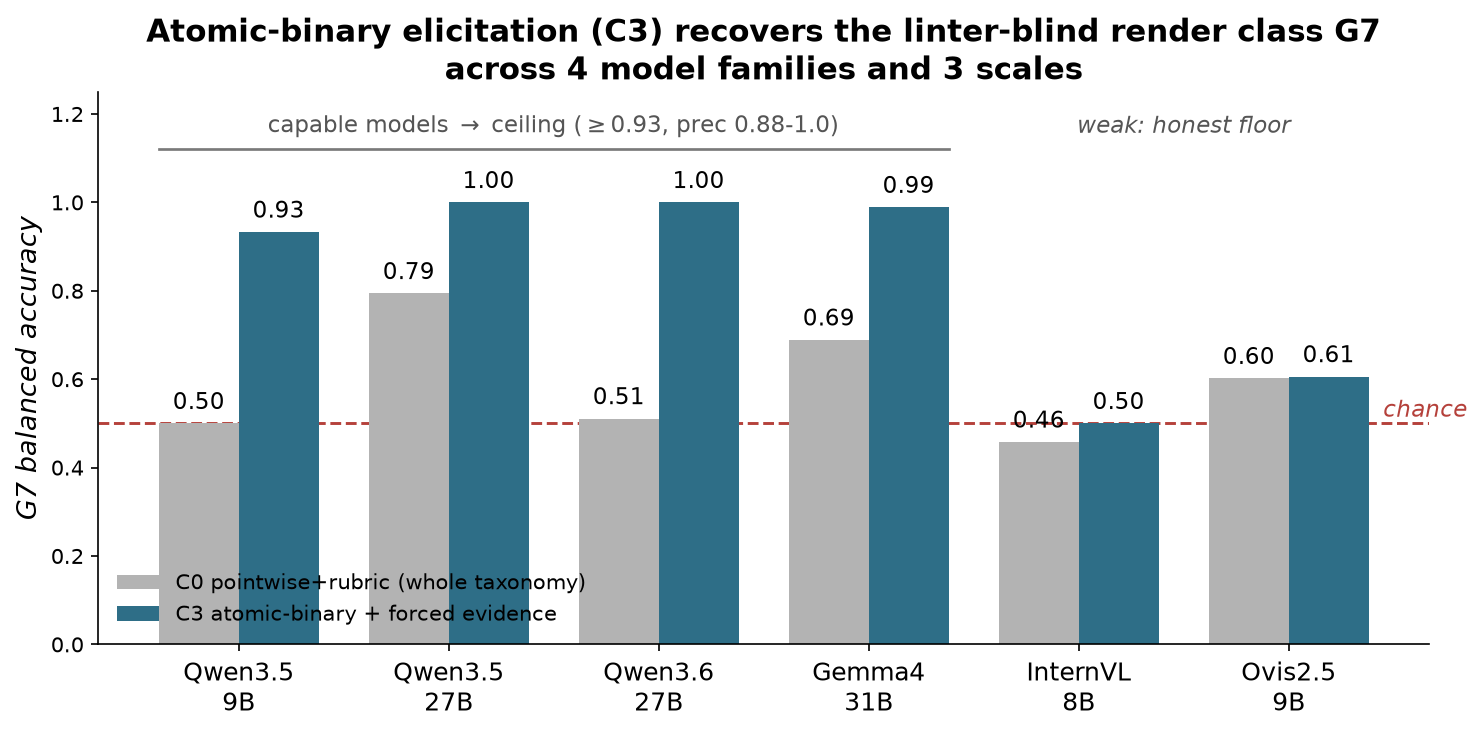
\includegraphics[width=0.8\linewidth]{figs/fig5_c3_vs_c0_g7.png}
\caption{\textbf{Atomic-binary elicitation (C3) recovers the linter-blind
render class \g{G7} across the capable subset} (referenced in \S5.1).
Capable models reach the ceiling ($\ge0.93$, precision 0.88--1.0); the weaker
InternVL/Ovis stay near their perceptual floor, a capability-dependent
boundary, not a universal fix.}
\label{figA:c3}
\end{figure}

\begin{figure}[h]
\centering
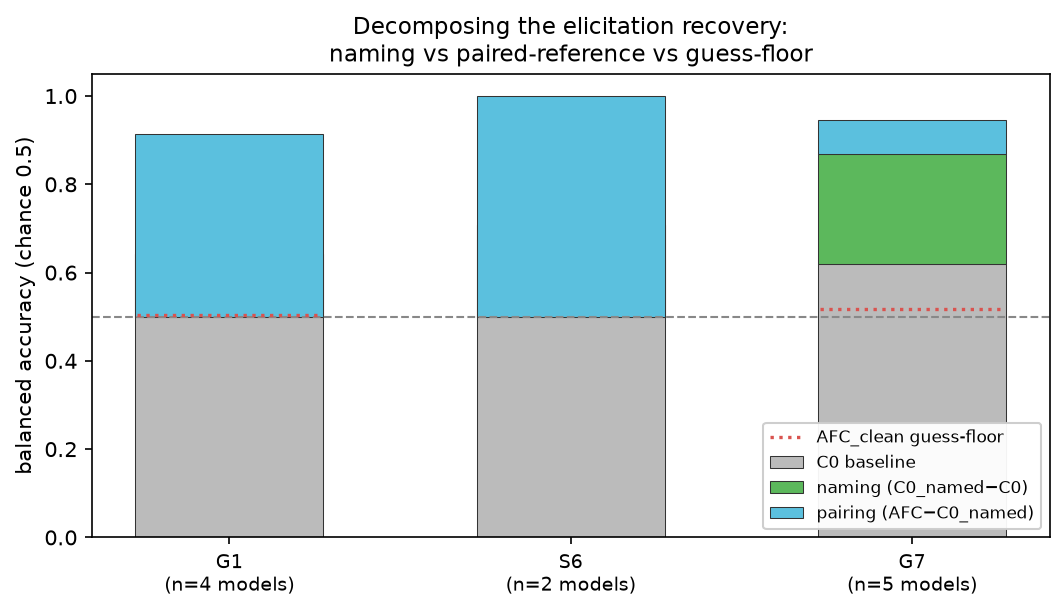
\includegraphics[width=0.78\linewidth]{figs/fig7_elicitation_decomp.png}
\caption{\textbf{What drives the recovery: naming vs.\ a paired reference}
(referenced in \S5.1). The chance$\to$ceiling jump factors into a
\emph{naming} component (C0\_named$-$C0) and a \emph{pairing} component
(AFC$-$C0\_named). For \g{G7} the naming term carries it (green); for \g{G1}
and \g{S6} the paired reference does (blue). The AFC\_clean guess-floor
(dotted) is near chance, so neither is a forced-pick artifact.}
\label{figA:decomp}
\end{figure}

\begin{figure}[h]
\centering
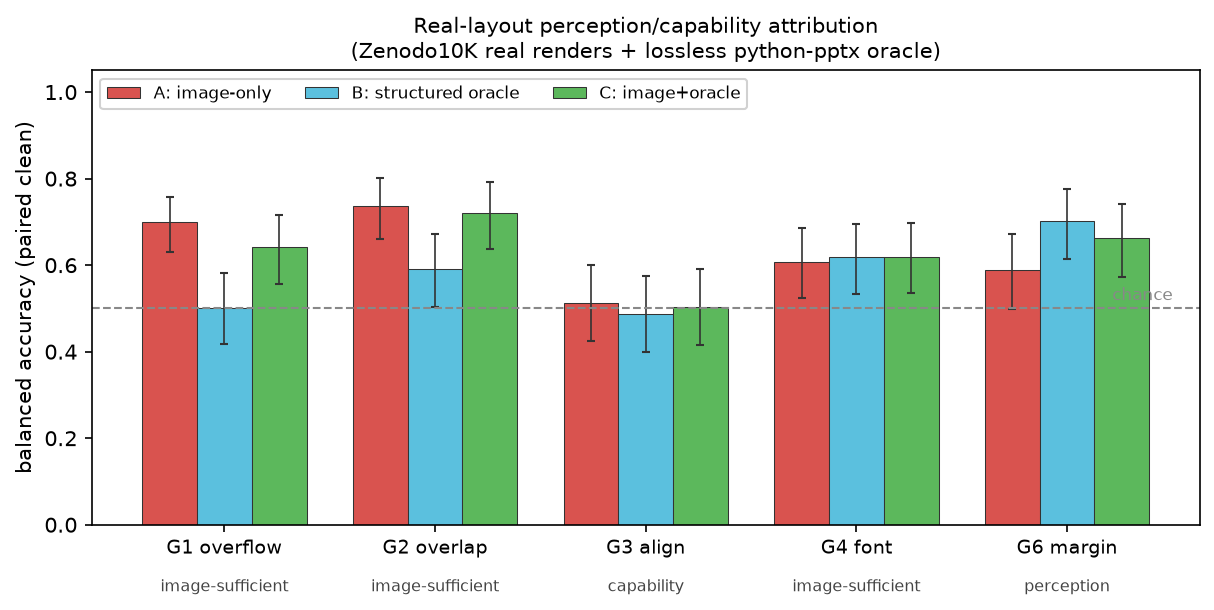
\includegraphics[width=0.75\linewidth]{figs/fig6_real_attribution.png}
\caption{\textbf{The perception/capability split reproduces on real layouts}
(referenced in \S7). \textsc{Zenodo10K} real renders + lossless
\texttt{python-pptx} oracle; mean over 3 VLMs / 3 families, balanced accuracy
on paired clean; 95\% Wilson on counts pooled across models ($n{=}76$--$90$
per class). Coarse defects are image-sufficient; \g{G6} margin is a perception
bottleneck the oracle rescues (B${>}$A); \g{G3} alignment stays near chance
in every channel on real cluttered decks.}
\label{figA:real}
\end{figure}

\begin{figure}[h]
\centering
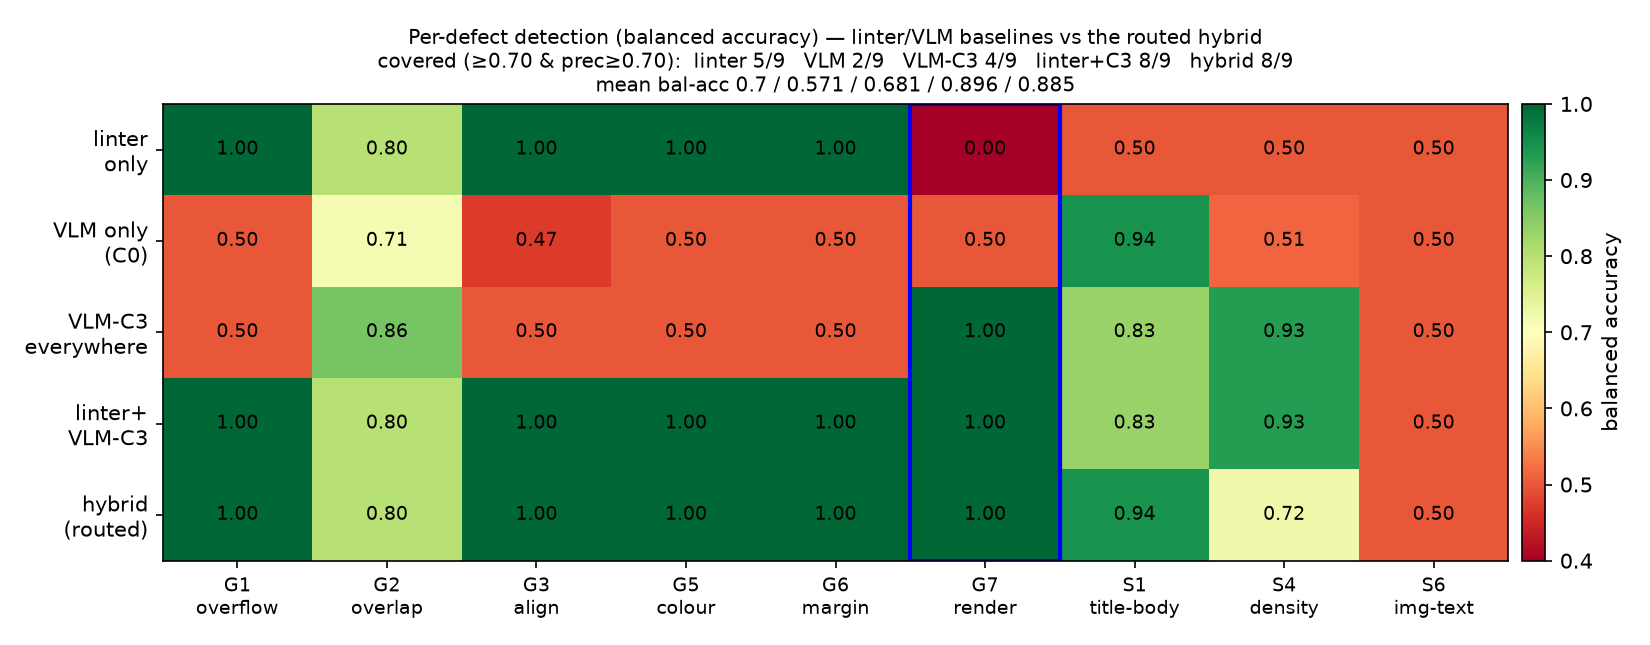
\includegraphics[width=0.7\linewidth]{figs/fig3_coverage_heatmap.png}
\caption{\textbf{Coverage by engine} (companion to Table~2 of the main paper).
Per-defect balanced accuracy for the linter, VLM-C0, VLM-C3, linter+VLM-C3,
and the routed hybrid. Minimal linter$\oplus$C3 has the highest mean balanced accuracy;
\g{G7} (boxed) is the linter-blind cell rescued by C3.}
\label{figA:coverage}
\end{figure}

\begin{figure}[h]
\centering
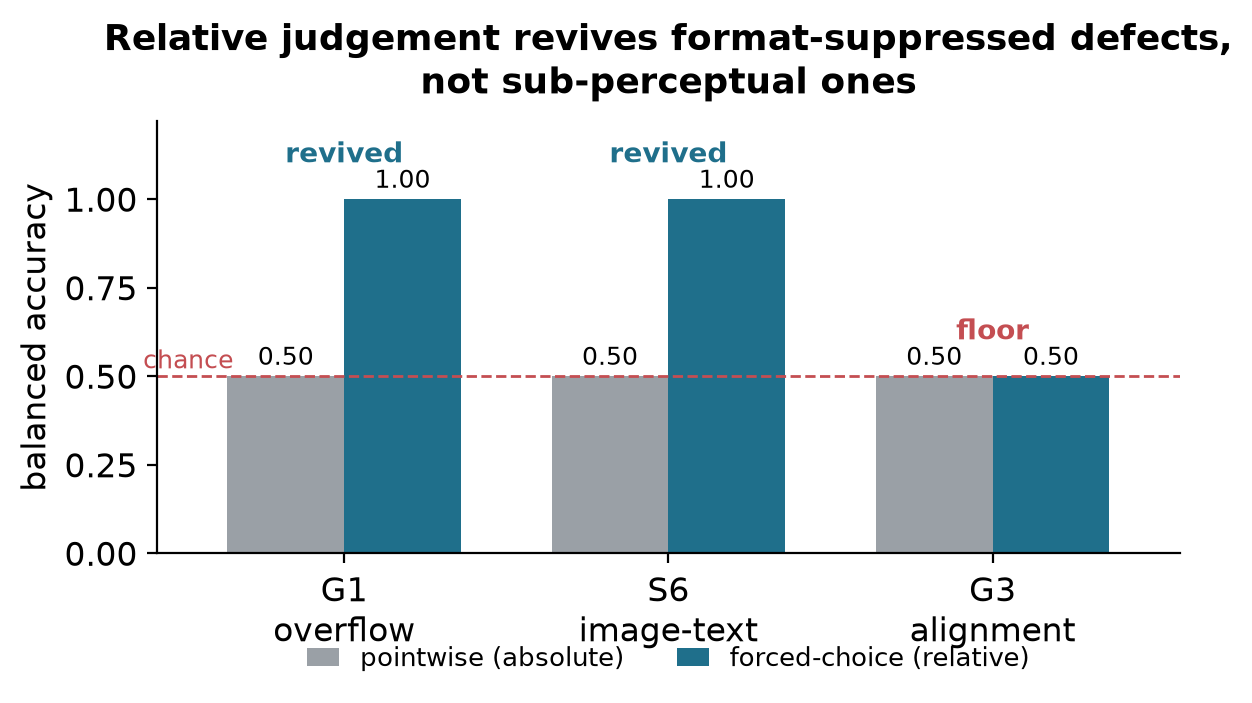
\includegraphics[width=0.7\linewidth]{figs/fig2_relative_vs_absolute.png}
\caption{\textbf{Relative judgement recovers absolute-pointwise blind spots}
(referenced in \S4). For \g{G1} overflow and \g{S6} image/text contradiction,
pointwise (absolute) inspection is at chance but a forced choice recovers
perfect detection. \g{G3} alignment behaves the same way above a magnitude
threshold; only its sub-threshold tail and \g{S3} terminology stay at chance
side by side.}
\label{figA:rel}
\end{figure}

% =====================================================================
\section{Conceptual figures}\label{app:concept}
% =====================================================================

These vector ``concept'' figures (with text overlays) were used in the
single-column technical report and are reproduced here for readers who prefer
the pictorial version of the protocol and routing arguments. They convey no
information beyond the body prose and the data figures above; they are
included for readability.

\begin{figure}[h]
\centering
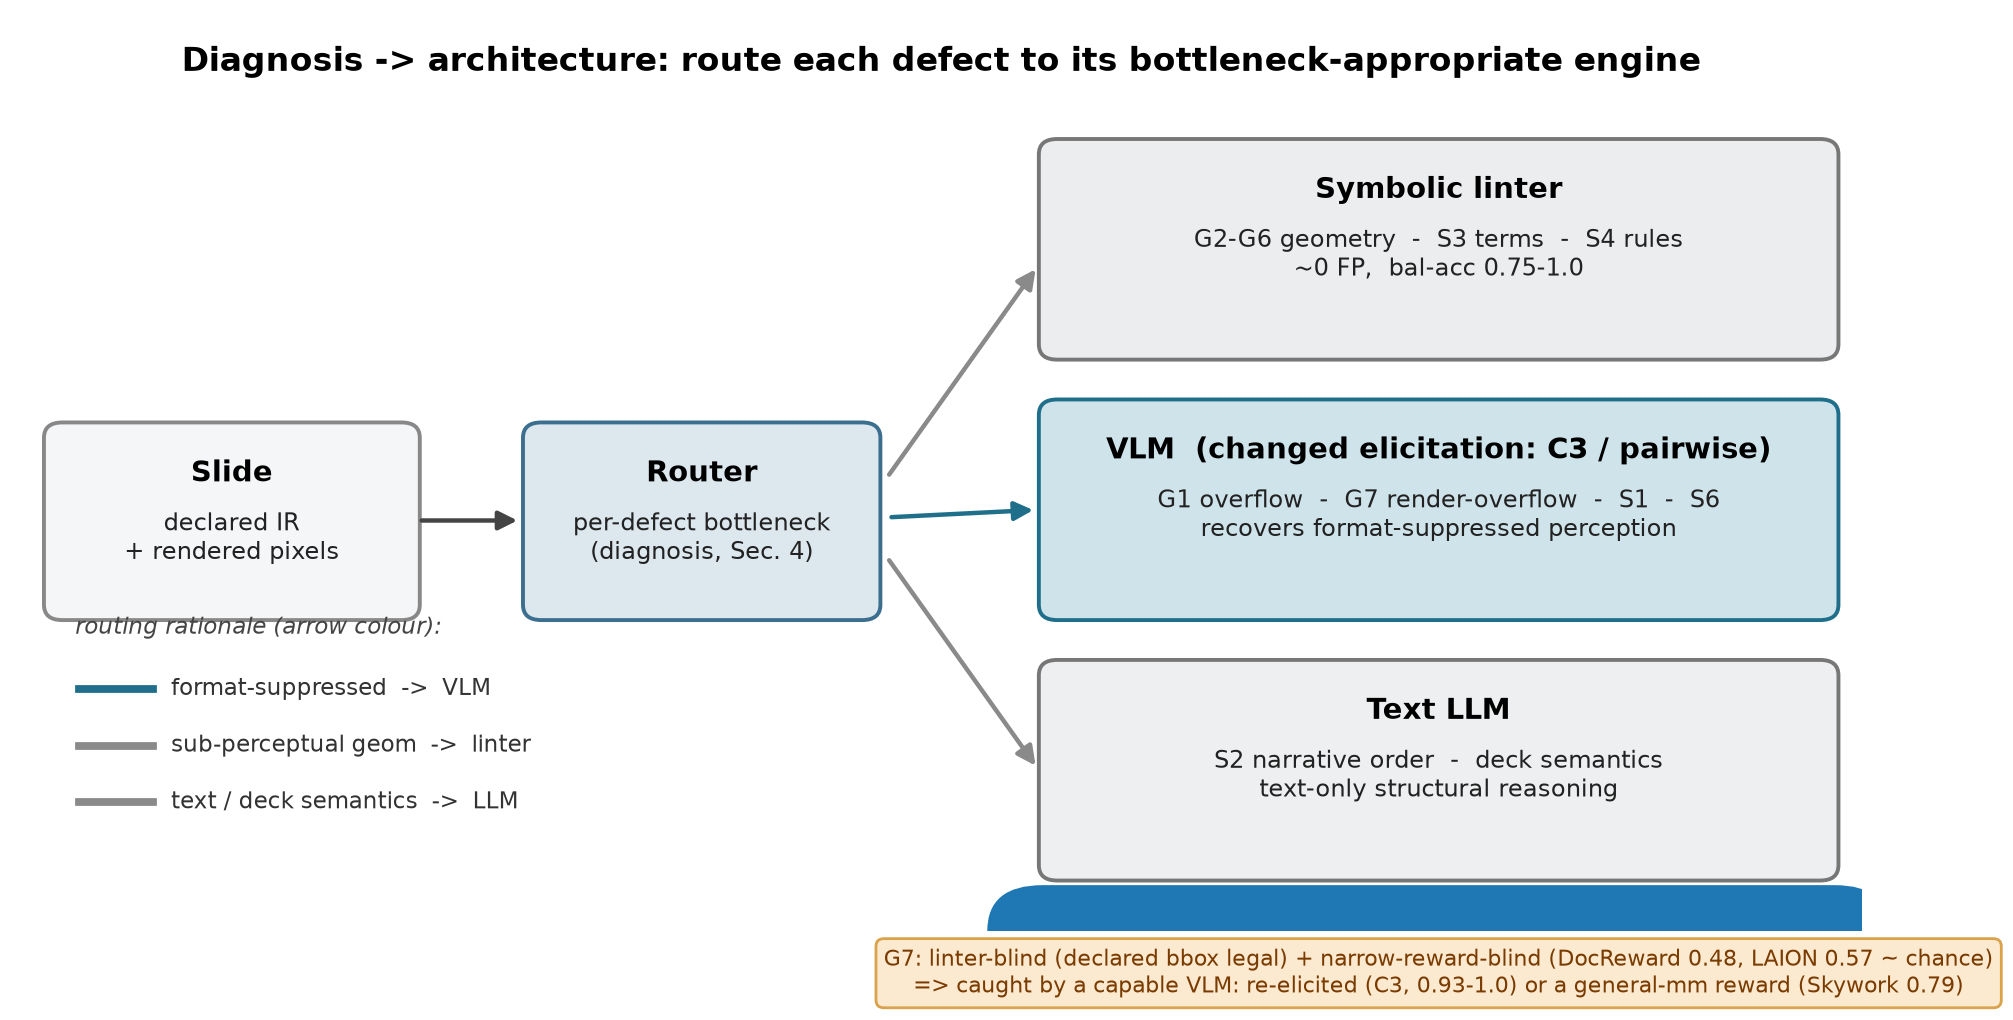
\includegraphics[width=0.95\linewidth]{figs/fig1_routing.png}
\caption{\textbf{Diagnosis $\to$ architecture.} Route each defect to the
engine that owns its bottleneck: declared geometry to a symbolic linter,
format-suppressed perceivable classes to a re-elicited VLM, text/deck
semantics to an LLM. The \g{G7} callout marks the linter-blind
render-overflow class caught only by an engine with a rendered-quality
read-out (Sec.~5 of the main paper). Companion to the teaser (Fig.~1).}
\label{figA:routing}
\end{figure}

\begin{figure}[h]
\centering
\begin{overpic}[width=0.9\linewidth,percent]{figs/fig_modality_task_notext.pdf}%
  \put(32.92,54.83){\makebox(0,0)[b]{\footnotesize\bfseries\color{figink} Detect}}
  \put(57.08,54.83){\makebox(0,0)[b]{\footnotesize\bfseries\color{figink} Localize}}
  \put(81.25,54.83){\makebox(0,0)[b]{\footnotesize\bfseries\color{figink} Repair}}
  \put(10.0,42.25){\makebox(0,0)[b]{\scriptsize\bfseries\color{figink} image-only}}
  \put(10.0,29.75){\makebox(0,0)[b]{\scriptsize\bfseries\color{figink} structured oracle}}
  \put(10.0,17.25){\makebox(0,0)[b]{\scriptsize\bfseries\color{figink} VLM-caption}}
  \put(10.0,4.75){\makebox(0,0)[b]{\scriptsize\bfseries\color{figink} image + oracle}}
\end{overpic}
\caption{\textbf{Attribution protocol.} Each paired (defective, clean) slide
is presented under four input modalities (image-only, the lossless structured
oracle, a fixed VLM-caption control, and image+oracle) crossed with
detect/localize/repair. Comparing image-only against the structured oracle
isolates a clean perception/reasoning split (Sec.~3 of the main paper).}
\label{figA:modtask}
\end{figure}

\begin{figure}[h]
\centering
\begin{overpic}[width=0.85\linewidth,percent]{figs/fig_g7_overflow_notext.pdf}%
  \put(25.42,4.17){\makebox(0,0)[b]{\footnotesize\color{figink} rendered text fits the box}}
  \put(74.58,4.17){\makebox(0,0)[b]{\footnotesize\color{figink} rendered pixels overflow the box}}
  \put(50.0,2.5){\makebox(0,0)[b]{\scriptsize\itshape\color{figslate} the linter sees two identical, legal declared boxes; it is blind to the difference by construction}}
\end{overpic}
\caption{\textbf{\g{G7} render-overflow.} The declared box (dashed) is legal
and \emph{identical} in both slides; only the rendered pixels overflow on the
right. The linter and any structure-only model read the same legal box in
both, so they are blind to \g{G7} by construction (Sec.~5.3 of the main
paper).}
\label{figA:g7concept}
\end{figure}

\begin{figure}[h]
\centering
\begin{overpic}[width=0.8\linewidth,percent]{figs/fig_rel_vs_abs_notext.pdf}%
  \put(25.42,43.33){\makebox(0,0)[b]{\small\bfseries\color{figink} absolute (pointwise)}}
  \put(25.42,36.67){\makebox(0,0){\large\bfseries\color{figslate} ?}}
  \put(25.42,7.67){\makebox(0,0)[b]{\scriptsize\itshape\color{figslate} score one slide alone $\rightarrow$ at chance for \g{G1}/\g{S6}}}
  \put(74.58,43.33){\makebox(0,0)[b]{\small\bfseries\color{figink} relative (forced choice)}}
  \put(74.58,7.67){\makebox(0,0)[b]{\scriptsize\itshape\color{figslate} compare a pair $\rightarrow$ recovers perfect detection}}
\end{overpic}
\caption{\textbf{Two elicitations, same model and images.} Pointwise (absolute)
inspects one slide in isolation; the forced choice compares a pair. For \g{G1}
and \g{S6}, changing absolute to relative is what recovers detection
(Sec.~4 of the main paper).}
\label{figA:relconcept}
\end{figure}

\begin{figure}[h]
\centering
\begin{overpic}[width=0.95\linewidth,percent]{figs/fig_openworld_notext.pdf}%
  \put(14.06,14.69){\makebox(0,0)[b]{\footnotesize\color{figslate} raw pixels (no IR)}}
  \put(34.77,17.34){\makebox(0,0)[b]{\footnotesize\color{figslate} layout parser}}
  \put(55.31,15.0){\makebox(0,0)[b]{\footnotesize\color{figslate} recovered structure}}
  \put(55.31,13.28){\makebox(0,0)[b]{\scriptsize\itshape\color{figgrey} (approximate, not native IR)}}
  \put(81.25,29.84){\makebox(0,0)[b]{\footnotesize\bfseries\color{figred} symbolic linter}}
  \put(81.25,28.12){\makebox(0,0)[b]{\scriptsize\itshape\color{figred} not restored}}
  \put(80.47,3.52){\makebox(0,0)[b]{\footnotesize\bfseries\color{figblue} re-elicited VLM}}
\end{overpic}
\caption{\textbf{Open world: recovered structure does not restore the linter.}
For bare third-party pixels with no IR, a layout parser recovers approximate
structure, but it is not the native IR the symbolic linter needs; only the
re-elicited VLM remains a deployable critic (Sec.~7 of the main paper).}
\label{figA:openconcept}
\end{figure}

\end{document}
